%%%%%%%%%%%%%%%%%%%%%%%%%%%%%%%%%%%%%%%%%%%%%%%%%%%%%%%%%%%%%%%%%%%%%%%%%%%%%%%%
%%% USE 80 character line lengths with linebreaks (Emacs-style)
%%%%%%%%%%%%%%%%%%%%%%%%%%%%%%%%%%%%%%%%%%%%%%%%%%%%%%%%%%%%%%%%%%%%%%%%%%%%%%%%

\documentclass[aip,jcp]{revtex4-1}

\usepackage{amsmath}
\usepackage{amssymb}
\usepackage{graphicx}
\usepackage[version=3]{mhchem}
\usepackage{physics}
\usepackage{xfrac} % gives \sfrac{}{}
\usepackage{gensymb} % \degree

\graphicspath{{./figures/}}

\newcommand{\dftbp}{DFTB+}

\renewcommand{\thetable}{S\arabic{table}}
\renewcommand{\theequation}{S\arabic{equation}}
\renewcommand{\thefigure}{S\arabic{figure}}
\renewcommand{\bibnumfmt}[1]{[S#1]}
\renewcommand{\citenumfont}[1]{S#1}

\begin{document}

\title{Supplementary Material for \\
  ``\dftbp{}, a software package for efficient approximate density functional
  theory based atomistic simulations``}

\maketitle

\section{Damping parameters for the D4-dispersion}

The recommended damping parameters for the freely available Slater--Koster sets
on \texttt{www.dftb.org} are listed in Tab.~\ref{stab:d4parameters}.
The damping parameters have been optimized to reproduce the interaction energies of the S66x8\cite{Rezac2011_S66x8}, S22x5\cite{grafova2010} and NCIBLIND10\cite{taylor2016} benchmark sets using a Levenberg--Marquardt algorithm.

\begin{table}[htbp]
  \caption{Becke--Johnson damping parameters for various Slater--Koster
    parametrizations of the DFTB hamiltonian. Parametrizations are done both
    with non-additive contributions and without.}
  \label{stab:d4parameters}
  \begin{tabular}{l*{5}{@{\qquad}c}}
    \hline
    \hline
    parameters & $s_6$ & $s_8$ & $s_9$ & $a_1$ & $a_2$ [$a_0$] \\
    \hline
    3ob
               & 1 & 0.4727337 & 0 & 0.5467502 & 4.4955068 \\
               & 1 & 0.6635015 & 1 & 0.5523240 & 4.3537076 \\
    matsci
               & 1 & 2.7711819 & 0 & 0.4681712 & 5.2918629 \\
               & 1 & 3.3157614 & 1 & 0.4826330 & 5.3811976 \\
    mio
               & 1 & 1.1948145 & 0 & 0.6074567 & 4.9336133 \\
               & 1 & 1.2916225 & 1 & 0.5965326 & 4.8778602 \\
    ob2(base)
               & 1 & 2.7611320 & 0 & 0.6037249 & 5.3900004 \\
               & 1 & 2.9692689 & 1 & 0.6068916 & 5.4476789 \\
    pbc
               & 1 & 1.7303734 & 0 & 0.5546548 & 4.7973454 \\
               & 1 & 2.1667394 & 1 & 0.5646391 & 4.9576353 \\
    \hline
    \hline
  \end{tabular}
\end{table}


\section{Damping parameters for the many-body and the Tkatchenko-Scheffler
  dispersion}

The recommended $\beta$ (MBD) and $s_{\rm R}$ (TS) values for the mio and 3ob parameter sets are listed in Table~\ref{stab:MBD_TS_rangeseparation}.
These have been obtained by minimizing the cost function
\begin{equation}
    F(p_{\rm rs}) = \mathrm{MARE_{int}}(p_{\rm rs}) + \mathrm{MARE_{geom}}(p_{\rm rs})
\end{equation}
for the S66x8 database~\cite{Rezac2011_S66x8}, where $\mathrm{MARE_{int}}(p_{\rm rs})$ is the mean absolute relative error in interaction energies at a range-separation (or damping) parameter $p_{\rm rs}$, \textit{i.e.}, $\beta$ for MBD and $s_{\rm R}$ for TS, and $\mathrm{MARE_{geom}}(p_{\rm rs})$ is the corresponding mean absolute relative error in equilibrium distances. The equilibrium distance for each dimer has thereby been estimated by the minimum of the spline-interpolated dissociation curve. In contrast to the previously reported optimization scheme,\cite{mortazavi2018} which inspired the current procedure, a more balanced and straightforward combination of energetic and geometric aspects based on relative errors has been used here. Figures~\ref{sfig:SI_TS_sR} and \ref{sfig:SI_MBD_beta} show a summary of the mean absolute errors and mean absolute relative errors in interaction energies and predicted equilibrium distances plus the cost function for DFTB in conjunction with the TS and MBD dispersion models as a function of the $s_{\rm R}$- and $\beta$-parameter, respectively.

\begin{table}[htbp]
  \centering
  \caption{Recommended MBD and TS range separation parameters for the mio and
    3ob parametrizations as obtained by minimizing the sum of absolute relative
    errors in interaction energies and predicted equilibrium distances for the
    S66x8 set\cite{Rezac2011_S66x8} of small molecular dimers.}
  \label{stab:MBD_TS_rangeseparation}
  \begin{tabular}{c c c}\hline\hline
    & ~~~MBD ($\beta$)~~~ & ~~~TS ($s_{\rm R}$)~~~ \\\hline
    3ob & 0.89 & 1.03 \\
    mio & 0.95 & 1.06 \\\hline\hline
  \end{tabular}
\end{table}

\begin{figure}[htbp]
    \centering
    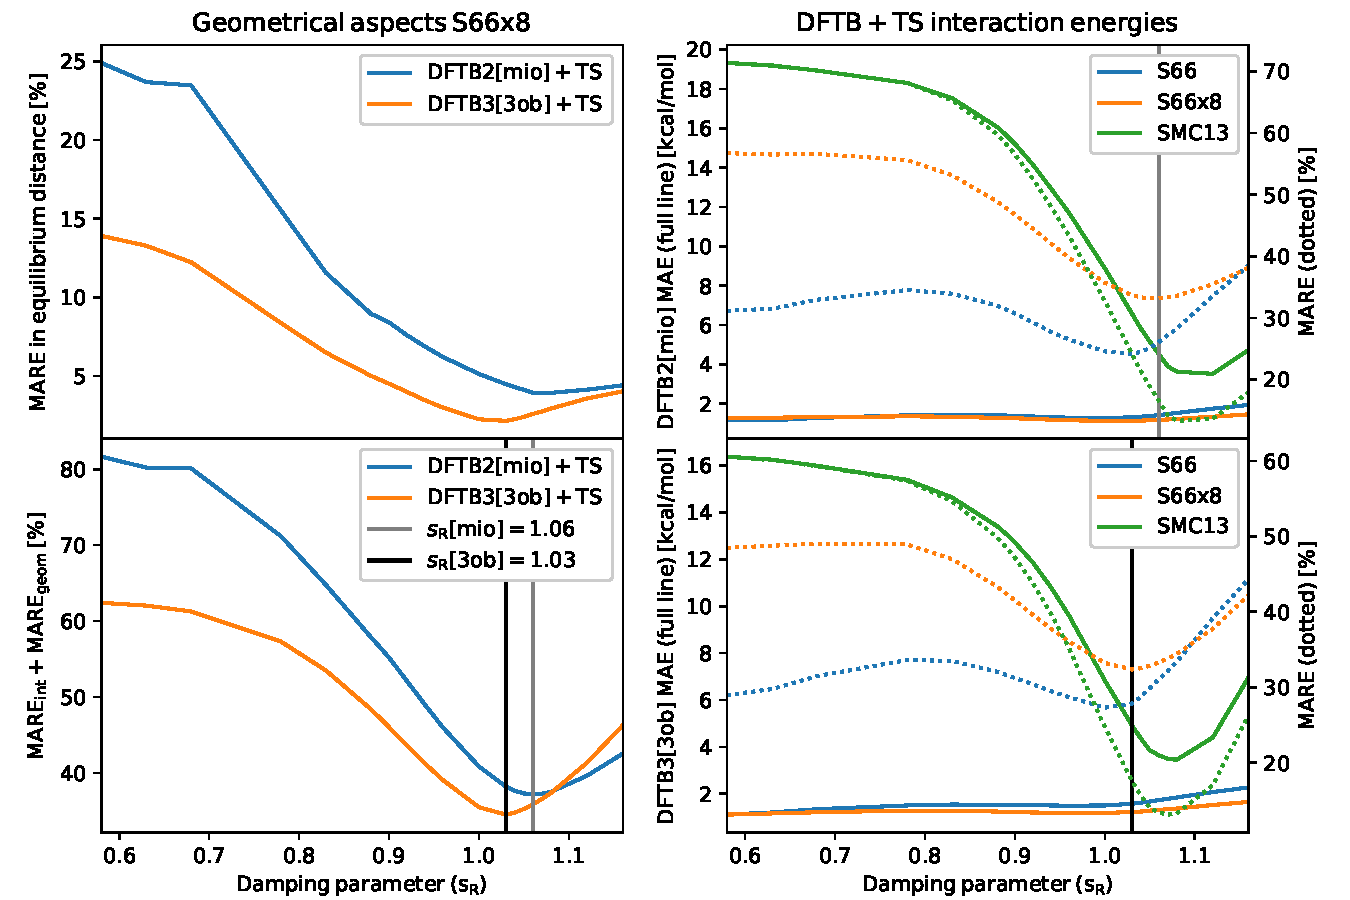
\includegraphics[scale=.66]{figures/SI_TSsR.pdf}
    \caption{Performance of DFTB2[mio] and DFTB3[3ob] in conjunction with the TS dispersion model as a function of the damping parameter $s_{\rm R}$. top left: equilibrium binding distances for the S66x8\cite{Rezac2011_S66x8} set. top tight: DFTB2[mio]+TS interaction energies for S66,\cite{Rezac2011_S66} S66x8, and SMC13.\cite{Ambrosetti2014_JPCL,Hermann2017,Stoehr2019_CSR} bottom left: cost function combining energetic and geometric aspects of S66x8. bottom right: DFTB3[3ob]+TS interaction energies for the S66, S66x8, and SMC13.}
    \label{sfig:SI_TS_sR}
\end{figure}
\begin{figure}[htbp]
    \centering
    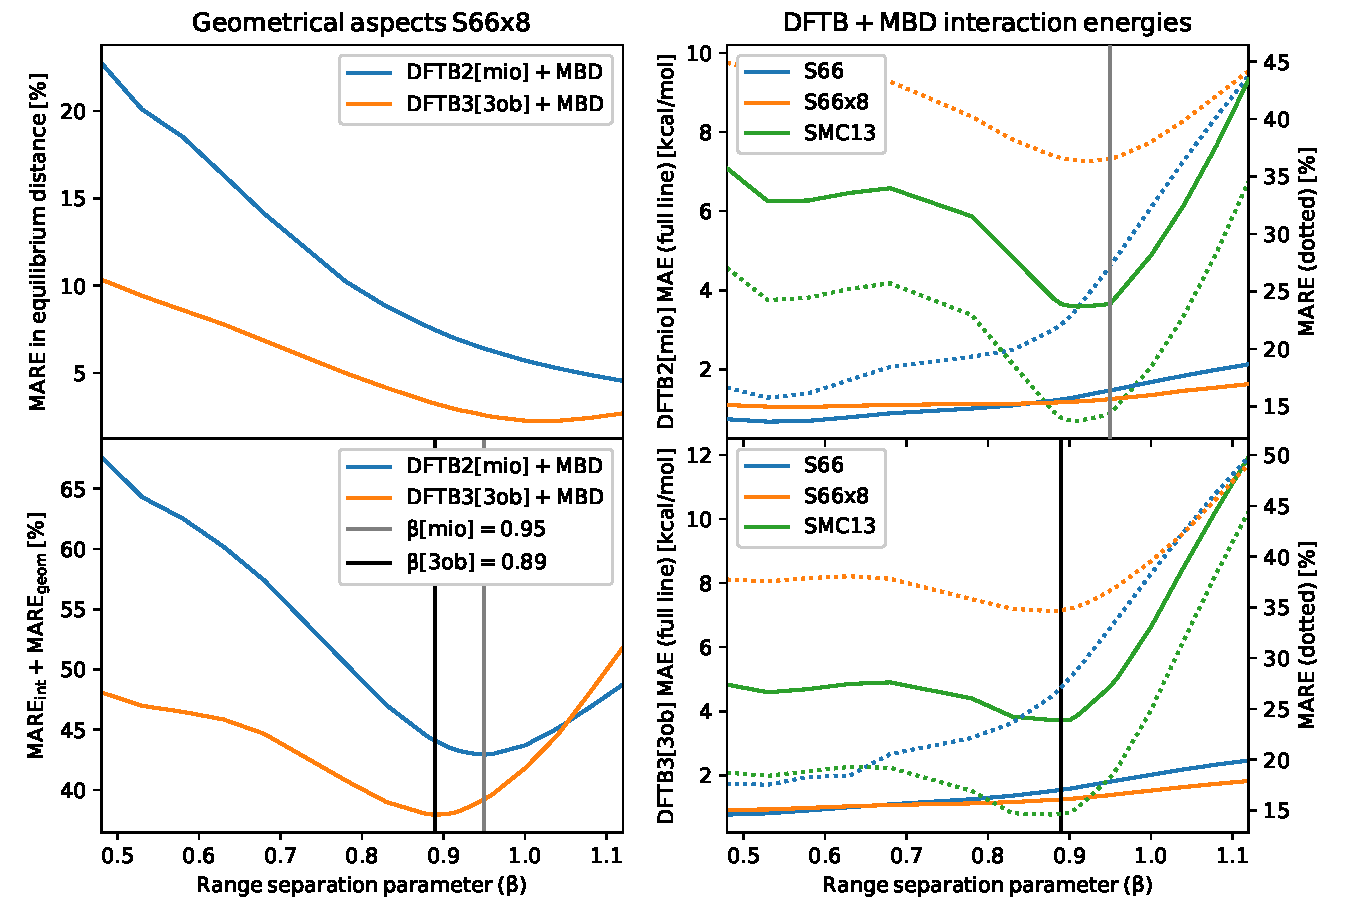
\includegraphics[scale=.66]{figures/SI_MBDbeta.pdf}
    \caption{Performance of DFTB2[mio] and DFTB3[3ob] in conjunction with the MBD dispersion model as a function of the range-separation parameter $\beta$. top left: equilibrium binding distances for the S66x8\cite{Rezac2011_S66x8} set. top tight: DFTB2[mio]+MBD interaction energies for S66,\cite{Rezac2011_S66} S66x8, and SMC13.\cite{Ambrosetti2014_JPCL,Hermann2017,Stoehr2019_CSR} bottom left: cost function combining energetic and geometric aspects of S66x8. bottom right: DFTB3[3ob]+MBD interaction energies for the S66, S66x8, and SMC13.}
    \label{sfig:SI_MBD_beta}
\end{figure}

\bibliographystyle{apsrev4-2}
\bibliography{titles,references}


\end{document}
